\documentclass[conference]{IEEEtran}
\IEEEoverridecommandlockouts

\usepackage{cite}
\usepackage{amsmath,amssymb,amsfonts}
\usepackage{graphicx}
\usepackage{booktabs}
\usepackage{multirow}
\usepackage{array}
\usepackage{tikz}
\usepackage{pgfplots}
\usepackage{pgfplotstable}
\usepackage{hyperref}
\usepackage{xurl}
\pgfplotsset{compat=1.18}
\usetikzlibrary{arrows.meta,positioning,fit,calc,shapes.geometric,backgrounds}

\definecolor{accentblue}{RGB}{62,95,138}
\definecolor{accentgreen}{RGB}{78,130,110}
\definecolor{accentorange}{RGB}{191,116,74}
\definecolor{softgray}{RGB}{115,122,128}

\tikzset{
box/.style={draw=softgray, rounded corners=2pt, thick, fill=gray!4, align=center, inner sep=6pt},
smallbox/.style={draw=softgray, rounded corners=2pt, thick, fill=gray!2, align=center, inner sep=4pt},
line/.style={-{Latex[length=2.2mm]}, thick, draw=softgray},
databox/.style={draw=softgray, rounded corners=2pt, thick, fill=blue!3, align=center, inner sep=5pt},
}

\title{Workload-Aware Multi-Objective Search for a Parameterized Kubernetes Scheduler}

\author{
\IEEEauthorblockN{Ismail Tarim}
\IEEEauthorblockA{
Izmir Katip Celebi University \\
Izmir, Turkiye \\
240401098@ogr.ikc.edu.tr
}
}

\begin{document}

\hypersetup{
  hidelinks,
  pdftitle={Workload-Aware Multi-Objective Search for a Parameterized Kubernetes Scheduler},
  pdfauthor={Ismail Tarim},
  pdfsubject={IEEE conference paper draft on Kubernetes scheduler policy optimization},
  pdfkeywords={Kubernetes scheduler, custom scheduler, evolutionary optimization, Pareto front, workload-aware scheduling}
}

\maketitle

\begin{abstract}
Kubernetes scheduling is a placement problem in which low queueing delay and efficient node usage are often competing goals. We present a live custom Kubernetes scheduler whose node-scoring policy is parameterized by four interpretable weights: \texttt{FreeCPU}, \texttt{FreeMem}, \texttt{PodPenalty}, and \texttt{Packing}. We formulate policy search as a multi-objective optimization problem over p95 pending time and maximum active node count, and we evaluate candidate policies under synthetic pressure workloads that expose CPU-, memory-, and fragmentation-driven tradeoffs. To search this policy space, we connect an evolutionary optimizer to a live evaluator that patches scheduler weights, waits for rollout completion, replays workloads, and collects cluster-level metrics. Our central question is whether, for controlled workload regimes, live-cluster multi-objective search can discover better tradeoff points than fixed hand-designed scheduler policies. On a 4-worker cluster, the Packing baseline cuts mean active nodes from $4$ to $2$ under both \texttt{cpu-tight} and \texttt{mem-tight}, while a \texttt{seed=42} search over $72$ candidates yields two unique combined Pareto points, including an optimizer-only lower-pending regime. These results show that scheduler policy weights materially affect behavior and that real-cluster multi-objective search can recover useful workload-aware tradeoffs.
\end{abstract}

\begin{IEEEkeywords}
Kubernetes scheduler, custom scheduler, evolutionary optimization, Pareto front, multi-objective optimization, workload-aware scheduling
\end{IEEEkeywords}

\section{Introduction}
Kubernetes scheduling decides where newly created Pods should run. That decision directly affects queueing delay, resource fragmentation, and how many worker nodes must remain active to serve a workload \cite{ref-borg-k8s}. In practice, these objectives conflict. A scheduler that spreads Pods aggressively may reduce waiting time by activating more nodes, while a scheduler that packs work into fewer nodes may improve consolidation at the cost of higher delay under pressure. Scheduler design is therefore a tradeoff problem rather than a search for a universally best heuristic.

This paper studies that tradeoff on a real Kubernetes deployment. Instead of treating scheduler behavior as fixed, we expose the node-scoring policy of a custom scheduler through four interpretable weights: \texttt{FreeCPU}, \texttt{FreeMem}, \texttt{PodPenalty}, and \texttt{Packing}. These weights make the policy surface small enough to search directly while still capturing distinct spread-oriented and packing-oriented behaviors.

Our goal is not to claim universal superiority over the default Kubernetes scheduler or any single hand-designed heuristic. The narrower question is whether, for controlled workload regimes, a parameterized scheduler policy can produce better tradeoff points than fixed hand-designed baselines. To answer that question, we run the scheduler inside a kind-based cluster, replay reproducible synthetic workloads, and evaluate policies against two explicit objectives: p95 pending time and maximum active node count. The reported baseline matrix already separates spread-oriented and packing-oriented regimes under resource pressure while preserving zero unschedulable Pods. We then attach this live evaluation loop to a multi-objective evolutionary search procedure that explores the policy space and reports Pareto-efficient tradeoffs.

The main contributions of the paper are as follows:
\begin{itemize}
\item We implement and deploy a custom Kubernetes scheduler in a reproducible kind-based cluster, including live feasibility filtering for node readiness, unschedulable state, taints, tolerations, and resource fit.
\item We define a four-weight node-scoring policy that turns scheduler behavior from a fixed heuristic into a compact searchable policy surface.
\item We build a live evaluation loop that couples workload replay, scheduler reconfiguration, rollout verification, and cluster-level metric collection on a running Kubernetes deployment rather than relying only on simulation.
\item We show that this search space exhibits meaningful Pareto tradeoffs and that evolutionary search can discover policy regimes beyond fixed hand-designed baselines.
\end{itemize}

\section{Background and Problem Statement}
Kubernetes scheduling can be viewed as a two-stage decision process. When a Pod is created without a bound node, the scheduler first identifies a feasible candidate set and then chooses one candidate according to its placement policy \cite{ref-k8s-scheduling}. Feasibility is not optional bookkeeping; it encodes the minimum conditions under which a placement is valid. In a realistic cluster, a node that is not \texttt{Ready}, is explicitly marked unschedulable, or carries a taint that the Pod does not tolerate should not be considered an eligible placement target \cite{ref-k8s-node-status,ref-k8s-taints}. Likewise, even a healthy node must be rejected if the Pod's resource request does not fit the node's remaining allocatable CPU or memory. Any policy optimization built on top of scheduling therefore has to operate \emph{after} these feasibility constraints have been applied.

This distinction matters for the present work. We do not optimize over arbitrary nodes in the cluster; we optimize how to rank nodes that already satisfy operational constraints. Concretely, the custom scheduler implemented in this paper filters candidate nodes according to readiness, the \texttt{unschedulable} flag, taint--toleration compatibility, and resource fit. Only the surviving nodes are scored by the parameterized policy. As a result, the search problem is not ``which invalid placements should be allowed,'' but ``how should a valid candidate set be prioritized under competing objectives.''

The optimization target is the scheduler policy itself. Let $\mathbf{w} = (w_{\mathrm{cpu}}, w_{\mathrm{mem}}, w_{\mathrm{pod}}, w_{\mathrm{pack}})$ denote the four policy weights used by the scoring function. For any fixed weight vector, the scheduler can be deployed, exercised on a workload suite, and measured using cluster-level outcomes. In this paper, those outcomes are summarized by two objectives:
\begin{equation}
\min \; f_1(\mathbf{w}) = \mathrm{AvgP95Pending}(\mathbf{w})
\end{equation}
\begin{equation}
\min \; f_2(\mathbf{w}) = \mathrm{AvgMaxActiveNodes}(\mathbf{w})
\end{equation}
where each objective is aggregated across the workload set used by the evaluator. The first objective captures tail scheduling delay, while the second acts as a proxy for node consolidation and operational cost.

These objectives are intentionally not collapsed into a single scalar fitness in the main analysis. A spread-oriented policy may improve pending time by activating more nodes, while a packing-oriented policy may reduce node usage at the cost of higher delay under pressure. This makes the problem naturally multi-objective and motivates Pareto analysis rather than a single ``best'' scheduler score. Our claim is therefore modest but concrete: for controlled workload regimes, a workload-aware evaluation loop can discover useful Pareto tradeoffs among parameterized scheduler policies. We do not claim that the resulting policies are universally better than the default Kubernetes scheduler across all clusters and workloads.

\begin{figure}[t]
\centering
\resizebox{\linewidth}{!}{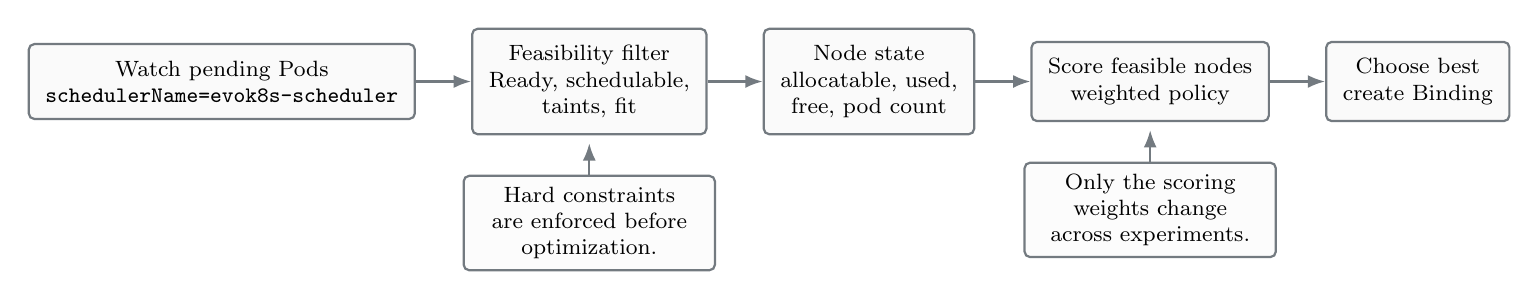
\begin{tikzpicture}[
  node distance=6mm and 7mm,
  every node/.style={font=\footnotesize}
]
\node[box, minimum width=0.18\linewidth] (watch) {Watch pending Pods\\\texttt{schedulerName=evok8s-scheduler}};
\node[box, right=of watch, minimum width=0.16\linewidth] (filter) {Feasibility filter\\Ready, schedulable,\\taints, fit};
\node[box, right=of filter, minimum width=0.15\linewidth] (state) {Node state\\allocatable, used,\\free, pod count};
\node[box, right=of state, minimum width=0.14\linewidth] (score) {Score feasible nodes\\weighted policy};
\node[box, right=of score, minimum width=0.13\linewidth] (bind) {Choose best\\create Binding};

\draw[line] (watch) -- (filter);
\draw[line] (filter) -- (state);
\draw[line] (state) -- (score);
\draw[line] (score) -- (bind);

\node[smallbox, below=5mm of filter, text width=0.24\linewidth] (note1) {Hard constraints are enforced before optimization.};
\node[smallbox, below=5mm of score, text width=0.24\linewidth] (note2) {Only the scoring weights change across experiments.};
\draw[line] (note1.north) -- ($(filter.south)+(0,-1mm)$);
\draw[line] (note2.north) -- ($(score.south)+(0,-1mm)$);
\end{tikzpicture}
}
\caption{Scheduler decision pipeline. The optimized policy operates only after feasibility filtering has reduced the candidate node set.}
\label{fig:scheduler-flow}
\end{figure}

\section{System Design}
The experimental platform is a real Kubernetes deployment built with kind \cite{ref-kind}. We use kind because it preserves the Kubernetes control-plane interfaces needed for scheduling experiments while remaining easy to recreate on a single machine. The cluster configurations used in this project are version-controlled, including the 4-worker topology used for the main resource-pressure experiments. This gives the study a controlled and repeatable testbed without reducing the system to a pure simulator.

The custom scheduler itself runs as a normal in-cluster deployment in the \texttt{evo-sched} namespace. A dedicated service account and cluster-wide RBAC policy grant the minimal permissions required for the scheduler to list Pods and Nodes and to create Pod bindings. The deployment injects the scheduler name and policy weights through environment variables, which allows the evaluator to reconfigure the policy without rebuilding the binary for each experiment. This deployment model is important methodologically: policy search interacts with the same mechanism that would be used to operate the scheduler in a real cluster.

At runtime, the scheduler uses in-cluster client credentials when running inside Kubernetes and falls back to the local kubeconfig only for out-of-cluster execution. The active scheduling loop polls unscheduled Pods using the field selector \texttt{spec.nodeName=} and processes only those whose \texttt{schedulerName} matches \texttt{evok8s-scheduler}. For each eligible Pod, the scheduler refreshes cluster state, builds a node resource snapshot from allocatable capacity and current Pod requests, filters infeasible nodes, scores the remaining candidates, and finally creates a Kubernetes \texttt{Binding} object for the selected node.

Two design choices are especially relevant for the credibility of the experiments. First, feasibility filtering is implemented in the live scheduler rather than approximated outside it: node readiness, explicit unschedulable state, taint--toleration compatibility, and resource fit are all checked before scoring. Second, the scheduling policy is separated cleanly from cluster orchestration. The binary always performs the same operational loop, while only the scoring weights change across experiments. This separation makes it possible to attribute observed behavior changes to policy differences rather than to different control logic.

The current implementation is intentionally simple in one respect: it follows a periodic scheduling loop with a two-second interval instead of implementing a full event-driven scheduler framework. That choice reduces engineering complexity for this project while preserving the essential live-cluster behavior needed for controlled policy evaluation. The resulting artifact is therefore best understood as a lightweight but real scheduler platform for workload-aware policy experiments.

\begin{figure*}[t]
\centering
\resizebox{0.93\textwidth}{!}{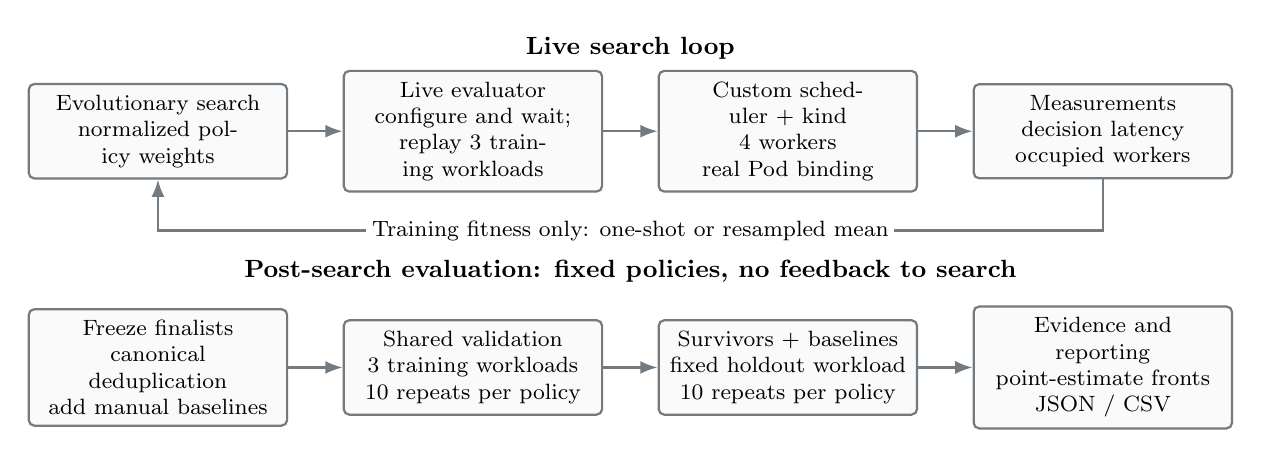
\begin{tikzpicture}[
  every node/.style={font=\footnotesize},
  stage/.style={box, text width=3.0cm, minimum height=1.15cm, inner sep=4pt},
  labeltext/.style={font=\footnotesize, align=center}
]
\node[stage] (optimizer) at (0,0) {Evolutionary search\\normalized policy weights};
\node[stage] (evaluator) at (4,0) {Live evaluator\\configure and wait;\\replay 3 training workloads};
\node[stage] (cluster) at (8,0) {Custom scheduler + kind\\4 workers\\real Pod binding};
\node[stage] (metrics) at (12,0) {Measurements\\decision latency\\occupied workers};
\draw[line] (optimizer) -- (evaluator);
\draw[line] (evaluator) -- (cluster);
\draw[line] (cluster) -- (metrics);
\draw[line] (metrics.south) -- ++(0,-0.65cm)
  -| (optimizer.south);
\node[labeltext, fill=white, inner sep=2pt]
  at ($(optimizer.south)!0.5!(metrics.south)+(0,-0.65cm)$)
  {Training fitness only: one-shot or resampled mean};
\node[labeltext, anchor=south, font=\small\bfseries]
  at ($(optimizer.north)!0.5!(metrics.north)+(0,0.18cm)$) {Live search loop};

\node[stage] (frozen) at (0,-3.0) {Freeze finalists\\canonical deduplication\\add manual baselines};
\node[stage] (validation) at (4,-3.0) {Shared validation\\3 training workloads\\10 repeats per policy};
\node[stage] (holdout) at (8,-3.0) {Survivors + baselines\\fixed holdout workload\\10 repeats per policy};
\node[stage] (report) at (12,-3.0) {Evidence and reporting\\point-estimate fronts\\JSON / CSV};
\draw[line] (frozen) -- (validation);
\draw[line] (validation) -- (holdout);
\draw[line] (holdout) -- (report);
\node[labeltext, anchor=south, font=\small\bfseries]
  at ($(frozen.north)!0.5!(report.north)+(0,0.18cm)$)
  {Post-search evaluation: fixed policies, no feedback to search};
\end{tikzpicture}
}
\caption{End-to-end architecture of the custom scheduler, evaluator, and optimizer pipeline. The evaluator reconfigures the live deployment, executes workloads on the cluster, and feeds measured outcomes back to the search procedure.}
\label{fig:system-architecture}
\end{figure*}

\section{Parameterized Scheduling Policy}
The optimized policy is a weighted node-scoring function defined over a compact per-node state representation. For each node, the scheduler records allocatable CPU and memory, the aggregate CPU and memory requests already assigned to the node, the resulting free capacity, and the number of non-terminal Pods currently placed there. These values are rebuilt from live cluster state before each scheduling pass, so the policy scores nodes using the same resource view that is available to the running scheduler.

The four policy signals are chosen to be both interpretable and operationally meaningful. \texttt{FreeCPU} rewards nodes with more available CPU capacity. \texttt{FreeMem} plays the same role for memory. \texttt{PodPenalty} discourages additional placements on nodes that already host many Pods, which biases the scheduler away from highly populated nodes even when resources remain available. \texttt{Packing} captures the opposite tendency: it rewards placements that leave less residual capacity after the candidate Pod is hypothetically assigned, thereby encouraging consolidation when feasible.

Let a node state be denoted by $s$, and let $r_{\mathrm{cpu}}$ and $r_{\mathrm{mem}}$ be the CPU and memory requests of the candidate Pod. The first two normalized terms are
\begin{equation}
\mathrm{freeCPU}(s) = \frac{\mathrm{FreeCPU}(s)}{\mathrm{AllocCPU}(s)},
\end{equation}
\begin{equation}
\mathrm{freeMem}(s) = \frac{\mathrm{FreeMem}(s)}{\mathrm{AllocMem}(s)}.
\end{equation}
To account for node population, the scheduler normalizes Pod count against the most populated feasible node in the current candidate set. Let
\begin{equation}
P_{\max} = \max_{s' \in \mathcal{F}} \mathrm{PodCount}(s').
\end{equation}
Then
\begin{equation}
\mathrm{podPenalty}(s) =
\left\{
\begin{aligned}
\frac{\mathrm{PodCount}(s)}{P_{\max}} & \quad \text{if } P_{\max} > 0,\\
0 & \quad \text{otherwise.}
\end{aligned}
\right.
\end{equation}
where $\mathcal{F}$ is the feasible node set after filtering.

The packing term is computed after a hypothetical placement of the candidate Pod on node $s$. If the remaining post-placement fractions are
\begin{equation}
\mathrm{remCPU}(s) = \frac{\max(0, \mathrm{FreeCPU}(s) - r_{\mathrm{cpu}})}{\mathrm{AllocCPU}(s)},
\end{equation}
\begin{equation}
\mathrm{remMem}(s) = \frac{\max(0, \mathrm{FreeMem}(s) - r_{\mathrm{mem}})}{\mathrm{AllocMem}(s)},
\end{equation}
then the normalized packing score is
\begin{equation}
\mathrm{packing}(s) = 1 - \frac{\mathrm{remCPU}(s) + \mathrm{remMem}(s)}{2}.
\end{equation}
This formulation assigns higher packing scores to nodes that would become more filled after placement, while still respecting the hard feasibility checks described earlier.

The final node score is a weighted linear combination:
\begin{equation}
\begin{aligned}
\mathrm{score}(s) =\;&
w_{\mathrm{cpu}} \cdot \mathrm{freeCPU}(s) +
w_{\mathrm{mem}} \cdot \mathrm{freeMem}(s) \\
&- w_{\mathrm{pod}} \cdot \mathrm{podPenalty}(s) +
w_{\mathrm{pack}} \cdot \mathrm{packing}(s).
\end{aligned}
\end{equation}
The scheduler chooses the feasible node with the highest score, breaking ties deterministically by node name. The search space is therefore the four-dimensional weight vector $\mathbf{w} = (w_{\mathrm{cpu}}, w_{\mathrm{mem}}, w_{\mathrm{pod}}, w_{\mathrm{pack}})$ rather than a large discrete space of hand-authored scheduling rules. This is the surface explored by the evolutionary search procedure in the next section.

\section{Evolutionary Policy Search}
The evolutionary search procedure treats each scheduler policy as an individual in a four-dimensional continuous search space. A candidate solution is simply the weight vector $\mathbf{w} = (w_{\mathrm{cpu}}, w_{\mathrm{mem}}, w_{\mathrm{pod}}, w_{\mathrm{pack}})$ introduced in the previous section. Evaluating an individual means deploying these weights to the running scheduler through the evaluator and measuring the resulting workload outcomes on the cluster. The optimizer therefore does not work with a surrogate model or synthetic fitness proxy; it searches directly against live cluster measurements.

The two optimization objectives are the aggregated outcomes returned by the evaluator:
\begin{equation}
\begin{aligned}
\min \; f_1(\mathbf{w}) &= \mathrm{AvgP95Pending}(\mathbf{w}), \\
\min \; f_2(\mathbf{w}) &= \mathrm{AvgMaxActiveNodes}(\mathbf{w}).
\end{aligned}
\end{equation}
Each objective is averaged over the workload set passed to the optimizer. In the current experiments, the optimizer evaluates three workloads---\texttt{cpu-tight}, \texttt{mem-tight}, and \texttt{fragmenting-mix}---so the search favors policies that perform well across multiple pressure regimes rather than overfitting to a single case.

The initial population is generated by sampling each weight independently from a bounded interval. In the implementation used here, the default search range is $[0, 2]$ for every weight and the initial population size is $12$. At each generation, offspring are created by tournament-selecting two parents from the current population, applying uniform crossover, and then applying per-gene Gaussian mutation. Uniform crossover means that each gene in the child is copied from one of the two parents with equal probability, while mutation perturbs each gene independently with probability $0.8$ using Gaussian noise with standard deviation $0.25$, followed by clamping back to the allowed weight interval.

Selection follows an NSGA-II-style elitist multi-objective procedure \cite{ref-nsga2}. After evaluating the offspring, the optimizer merges the parent and child populations, computes nondominated fronts, assigns crowding distance within each front, and then fills the next generation by rank and crowding priority. Tournament selection also uses this ordering: lower-rank candidates are preferred, and crowding distance breaks ties in favor of more isolated solutions. This mechanism simultaneously preserves high-quality tradeoff points and discourages premature collapse onto a single narrow region of the objective space.

One methodological detail is important for interpretation. The hand-designed baseline policies are evaluated by the same cluster-level loop, but they are not injected into the reproductive population. They serve as reference points for the final combined Pareto analysis rather than as seed individuals for crossover and mutation. This keeps the optimizer responsible for discovering its own tradeoff regimes while still allowing direct comparison against meaningful manually specified scheduler behaviors.

The experiments reported in this paper use a population size of $12$ and $5$ generations, which yields $72$ optimizer-evaluated candidates after the initial population and offspring generations, in addition to the separately evaluated baselines. Multiple random seeds are planned to test stability of the observed Pareto structure; the first complete run uses \texttt{seed=42}, and the remaining planned seeds are \texttt{123} and \texttt{999}.

Optimizer hyperparameters were not themselves treated as a separate tuning problem in this study. They were chosen as reasonable first-pass settings for a small search space with expensive real-cluster evaluation. In particular, the relatively high mutation probability is intentional: with only four genes and costly fitness evaluation, maintaining exploration is more valuable than aggressively exploiting early population structure. A more exhaustive sensitivity analysis over mutation rate, mutation scale, and population size remains future work.

\section{Evaluation Methodology and Experimental Setup}
\textit{Evaluator.} The evaluator is the component that turns a policy weight vector into measured outcomes. For each run, it reads the current scheduler deployment, stores the active weights, patches the deployment with the candidate weight set, waits for rollout completion, and then replays one or more workload files into a dedicated evaluator namespace. During execution it records Pod creation, scheduling, start, and completion timestamps, as well as the number of active worker nodes sampled over time. After the run, it summarizes the resulting Pod timings, cleans evaluator-managed Pods if cleanup is enabled, and restores the scheduler deployment to its original weight configuration. This reset step is essential for preventing cross-run contamination.

\textit{Workload model.} A workload is a time-ordered list of Pod descriptions. Each item specifies a Pod name, arrival time in seconds, CPU request, memory request, and runtime duration. The evaluator supports both absolute resource requests and fractional requests relative to the current worker-node capacity. Fractional workloads were introduced because they make the scenarios portable across cluster topologies: when a worker's allocatable capacity changes, the intended pressure profile is preserved by resolving fractions against the minimum allocatable CPU and memory observed across schedulable worker nodes.

\textit{Cluster setup.} The main experiments use a kind cluster with one control-plane node and four worker nodes. The custom scheduler runs as the \texttt{evok8s-scheduler} deployment in namespace \texttt{evo-sched}, while evaluator-created Pods run in the separate namespace \texttt{evo-sched-eval}. The scheduler image is configured once and then re-parameterized through environment variables, so repeated experiments differ only in policy weights and workload definitions.

\textit{Baselines.} Three hand-designed custom-scheduler baselines are used in the current study. For readability, we refer to them as \emph{Default}, \emph{Spread}, and \emph{Packing}; Table~\ref{tab:baseline-weights} maps these paper-facing names to their exact deployments and weight assignments. The three policies intentionally represent different regions of the search space: a neutral default setting, a spread-oriented regime that emphasizes free capacity and Pod-count avoidance, and a packing-oriented regime that rewards consolidation. The default Kubernetes scheduler is discussed as an external reference point, but it is not yet included as a fully experimental baseline in the current result tables.

\textit{Workload families.} The three main pressure workloads are \texttt{cpu-tight}, \texttt{mem-tight}, and \texttt{fragmenting-mix}. The first two isolate CPU-dominant and memory-dominant pressure by requesting approximately $45\%$ of worker capacity in one dominant resource dimension. The mixed workload combines CPU-heavy, memory-heavy, and balanced Pods in short bursts so that packing and spreading interact with fragmentation. This workload family proved most informative in the exploratory experiments because it exposes clear tradeoffs between low pending time and low node usage.

\textit{Metrics and repetition protocol.} The primary objectives are p95 pending time and maximum active node count. Pending time is measured as the time between Pod creation and the moment the Pod receives a node assignment; the reported p95 is computed over scheduled Pods only. Maximum active node count is the largest number of worker nodes simultaneously hosting evaluator-managed Pods during a run. We also record scheduled count, completed count, and unschedulable count as supporting metrics to ensure that node consolidation is not achieved by simply failing to place Pods. For the baseline matrix experiments, each workload--policy combination is repeated three times. For the optimizer, repeated runs are organized by random seed, with \texttt{42}, \texttt{123}, and \texttt{999} selected as the planned seed set. Load variance is a plausible additional metric, but because it is not yet part of the final result tables, it is treated as future work rather than as a primary evaluated quantity.

\begin{table}[t]
\caption{Experimental setup used for the main reported runs.}
\label{tab:setup}
\centering
\begin{tabular}{p{0.18\linewidth} p{0.72\linewidth}}
\toprule
Item & Value \\
\midrule
Cluster & kind, 1 control-plane + 4 workers \\
Scheduler & \texttt{evok8s-scheduler} custom deployment \\
Baselines & Default, Spread, and Packing; see Table~\ref{tab:baseline-weights} \\
Workloads & cpu-tight, mem-tight, fragmenting-mix \\
Objectives & average p95 pending, average max active nodes \\
Support metrics & scheduled, completed, unschedulable counts \\
Repeats & 3 per workload--baseline combination \\
Seeds & 42 completed; 123 and 999 planned \\
\bottomrule
\end{tabular}
\end{table}

\begin{table}[t]
\caption{Exact weight assignments for the three fixed baseline policies. The paper-facing names map to deployments \texttt{evok8s-default}, \texttt{evok8s-spread-heavy}, and \texttt{evok8s-packing-heavy}.}
\label{tab:baseline-weights}
\centering
\scriptsize
\begin{tabular}{lcccc}
\toprule
Policy & CPU & Mem & Pod & Pack \\
\midrule
Default & 1.0 & 1.0 & 0.5 & 0.2 \\
Spread & 1.4 & 1.4 & 1.0 & 0.0 \\
Packing & 0.5 & 0.5 & 0.2 & 1.3 \\
\bottomrule
\end{tabular}
\end{table}

\section{Results}
We report results in two stages. First, we compare the hand-designed baseline policies on the 4-worker resource-pressure workloads to establish whether the parameterized policy surface actually produces different scheduling behavior. Second, we analyze the first full optimizer run (\texttt{seed=42}) to determine whether evolutionary search finds Pareto tradeoff points beyond the hand-picked baseline set.

\subsection{Baseline Policy Comparison}
Table~\ref{tab:baseline-results} summarizes the 4-worker resource-pressure matrix. Across all reported baseline runs, every Pod was scheduled and completed successfully, and the unschedulable count remained zero. This is useful context: the observed node-usage reductions are not achieved by silently dropping workload demand.

The baseline comparison reveals that policy weights materially affect behavior under pressured workloads. The clearest pattern, visible in Table~\ref{tab:baseline-results} and Fig.~\ref{fig:baseline-nodes}, is that Packing consistently reduces node usage. Under both \texttt{cpu-tight} and \texttt{mem-tight}, it cuts the mean maximum active-node count from $4$ to $2$. Under \texttt{fragmenting-mix}, it still reduces node usage, but only to $3$, indicating that the mixed workload partially resists aggressive consolidation.

The delay-side story, shown in Fig.~\ref{fig:baseline-pending}, is more workload-dependent. Under \texttt{cpu-tight}, both Spread and Packing improve mean p95 pending from $2.00$ to $1.67$ relative to Default. Under \texttt{mem-tight}, all three baselines achieve the same mean p95 pending ($1.67$), but Packing does so with only half as many active nodes. Under \texttt{fragmenting-mix}, Spread and Packing achieve the same mean p95 pending, but Packing does so with fewer active nodes, reducing the mean maximum active-node count from $4$ to $3$. This confirms that the problem behaves as a real tradeoff surface rather than a single dominant heuristic regime.

Two conclusions follow from this matrix. First, the four policy weights are not cosmetic parameters; they generate distinct operational behaviors. Second, the active-node objective becomes visible only under sufficiently pressured workloads and a sufficiently large cluster. Earlier light-load experiments on the smaller cluster did not expose this separation nearly as clearly.

\begin{table*}[t]
\caption{Baseline comparison on the 4-worker resource-pressure workloads. Reported values are means across three repeats; all combinations produced zero unschedulable Pods.}
\label{tab:baseline-results}
\centering
\begin{tabular}{l l r r r}
\toprule
Workload & Policy & Mean p95 pending (s) & Mean max active nodes & Unschedulable \\
\midrule
\texttt{cpu-tight} & Default & 2.00 & 4.00 & 0 \\
\texttt{cpu-tight} & Spread & 1.67 & 4.00 & 0 \\
\texttt{cpu-tight} & Packing & 1.67 & 2.00 & 0 \\
\texttt{mem-tight} & Default & 1.67 & 4.00 & 0 \\
\texttt{mem-tight} & Spread & 1.67 & 4.00 & 0 \\
\texttt{mem-tight} & Packing & 1.67 & 2.00 & 0 \\
\texttt{fragmenting-mix} & Default & 2.00 & 4.00 & 0 \\
\texttt{fragmenting-mix} & Spread & 1.67 & 4.00 & 0 \\
\texttt{fragmenting-mix} & Packing & 1.67 & 3.00 & 0 \\
\bottomrule
\end{tabular}
\end{table*}

\begin{figure}[t]
\centering
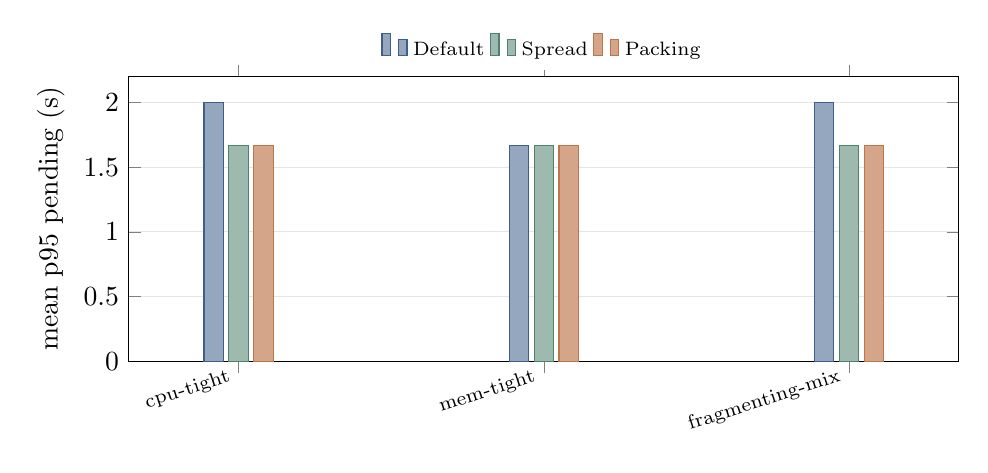
\begin{tikzpicture}
\begin{axis}[
  width=\linewidth,
  height=5.2cm,
  ybar,
  bar width=7pt,
  ymin=0,
  ymax=2.2,
  ylabel={mean p95 pending (s)},
  symbolic x coords={cpu-tight,mem-tight,fragmenting-mix},
  xtick=data,
  xticklabel style={rotate=18, anchor=east, font=\scriptsize},
  ymajorgrids=true,
  grid style={gray!20},
  legend style={font=\scriptsize, at={(0.5,1.02)}, anchor=south, legend columns=3, draw=none},
  enlarge x limits=0.18,
]
\addplot+[fill=accentblue!55, draw=accentblue] coordinates {
  (cpu-tight,2.00)
  (mem-tight,1.67)
  (fragmenting-mix,2.00)
};
\addplot+[fill=accentgreen!55, draw=accentgreen] coordinates {
  (cpu-tight,1.67)
  (mem-tight,1.67)
  (fragmenting-mix,1.67)
};
\addplot+[fill=accentorange!65, draw=accentorange] coordinates {
  (cpu-tight,1.67)
  (mem-tight,1.67)
  (fragmenting-mix,1.67)
};
\legend{Default,Spread,Packing}
\end{axis}
\end{tikzpicture}

\caption{Mean p95 pending time across the three baseline policies for each resource-pressure workload. Values are means across three repeats.}
\label{fig:baseline-pending}
\end{figure}

\begin{figure}[t]
\centering
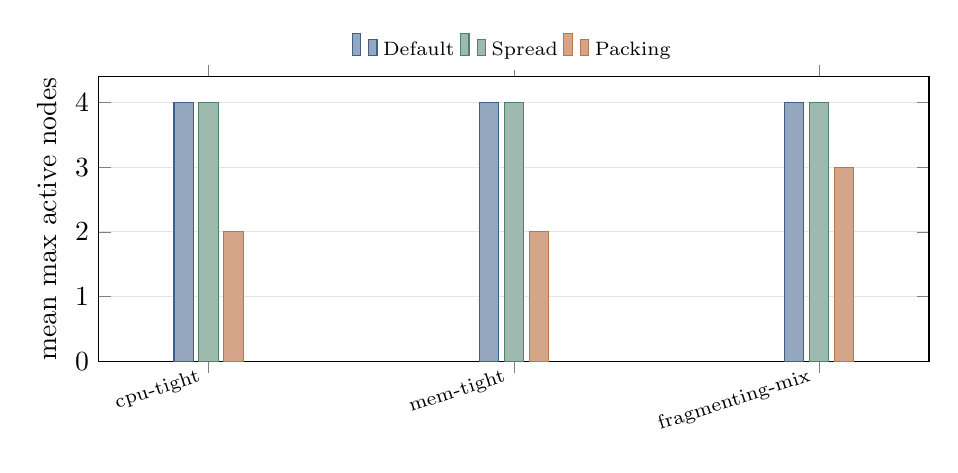
\begin{tikzpicture}
\begin{axis}[
  width=\linewidth,
  height=5.2cm,
  ybar,
  bar width=7pt,
  ymin=0,
  ymax=4.4,
  ylabel={mean max active nodes},
  symbolic x coords={cpu-tight,mem-tight,fragmenting-mix},
  xtick=data,
  xticklabel style={rotate=18, anchor=east, font=\scriptsize},
  ymajorgrids=true,
  grid style={gray!20},
  legend style={font=\scriptsize, at={(0.5,1.02)}, anchor=south, legend columns=3, draw=none},
  enlarge x limits=0.18,
]
\addplot+[fill=accentblue!55, draw=accentblue] coordinates {
  (cpu-tight,4.00)
  (mem-tight,4.00)
  (fragmenting-mix,4.00)
};
\addplot+[fill=accentgreen!55, draw=accentgreen] coordinates {
  (cpu-tight,4.00)
  (mem-tight,4.00)
  (fragmenting-mix,4.00)
};
\addplot+[fill=accentorange!65, draw=accentorange] coordinates {
  (cpu-tight,2.00)
  (mem-tight,2.00)
  (fragmenting-mix,3.00)
};
\legend{Default,Spread,Packing}
\end{axis}
\end{tikzpicture}

\caption{Mean maximum active-node count across the three baseline policies for each resource-pressure workload. Values are means across three repeats.}
\label{fig:baseline-nodes}
\end{figure}

\subsection{Pareto Front Analysis}
The first complete optimizer run uses population size $12$, $5$ generations, and \texttt{seed=42}. It evaluates $72$ optimizer-generated candidates and, with the three baselines, yields $75$ measured solutions. Unlike the three-repeat matrix in Table~\ref{tab:baseline-results}, these Pareto objectives come from the single optimizer evaluation stream. The combined front contains $4$ nondominated members but only $2$ \emph{unique} objective points, so we report unique coordinates rather than duplicate representatives.

For \texttt{seed=42}, the two unique combined Pareto points are $(0.67, 4.00)$ and $(1.00, 2.33)$ in the objective space of average p95 pending and average maximum active nodes. Figure~\ref{fig:pareto-seed42} shows this structure: one point is optimizer-only, while the other coincides with the Packing baseline. Rather than producing a dense cloud of incomparable solutions, the first run collapses onto two dominant regimes: lower pending or stronger consolidation.

\begin{figure}[t]
\centering
\begin{tikzpicture}
\begin{axis}[
  width=\linewidth,
  height=5.15cm,
  xmin=0.5,
  xmax=2.4,
  ymin=1.8,
  ymax=4.25,
  xtick={0.5,1.0,1.5,2.0},
  xlabel={average p95 pending (s)},
  ylabel={average max active nodes},
  grid=both,
  grid style={gray!18},
  minor grid style={gray!10},
  tick label style={font=\scriptsize},
  label style={font=\small},
  clip=false,
  legend style={
    font=\tiny,
    at={(0.97,0.06)},
    anchor=south east,
    legend columns=1,
    draw=none,
    fill=white,
    fill opacity=0.9,
    text opacity=1,
    cells={anchor=west}
  },
  legend image post style={scale=0.72},
]
\addplot[
  only marks,
  mark=*,
  mark size=1.2pt,
  draw=gray!60,
  fill=gray!55,
  opacity=0.45,
] table[
  col sep=comma,
  x=avg_p95_pending,
  y=avg_max_active_nodes
] {../results/2026-03-15-optimizer-seed42/result-all.csv};
\addlegendentry{all measured solutions}

\addplot[
  only marks,
  mark=square*,
  mark size=2.6pt,
  draw=accentblue,
  fill=accentblue!75,
] coordinates {
  (1.666667,4.000000)
  (1.000000,4.000000)
  (1.000000,2.333333)
};
\addlegendentry{baseline policies}

\addplot[
  only marks,
  mark=*,
  mark size=3.8pt,
  draw=accentorange,
  fill=accentorange!85,
] coordinates {
  (0.666667,4.000000)
  (1.000000,2.333333)
};
\addlegendentry{unique Pareto points}

\node[
  font=\scriptsize\bfseries,
  anchor=south west,
  fill=white,
  rounded corners=1pt,
  inner sep=0.8pt,
  text=accentorange!85!black
] at (axis cs:0.72,4.02) {A};

\node[
  font=\scriptsize\bfseries,
  anchor=south west,
  fill=white,
  rounded corners=1pt,
  inner sep=0.8pt,
  text=accentorange!85!black
] at (axis cs:1.04,2.36) {B};
\end{axis}
\end{tikzpicture}

\caption{Seed-42 Pareto front. Gray: all measured solutions; blue: baselines; orange: unique Pareto points. A is optimizer-only; B coincides with Packing.}
\label{fig:pareto-seed42}
\end{figure}

\subsection{Optimizer-Discovered Policies}
The optimizer contributes two important findings. First, not all hand-designed baselines survive Pareto comparison. In the combined front, Packing remains nondominated, while Default and Spread are dominated. This means the default custom-policy setting is not a robust compromise policy for the selected workloads, and the spread-oriented heuristic does not remain Pareto-optimal once nearby regions of the policy space are explored.

Second, the optimizer discovers a genuinely new lower-pending Pareto regime. Two generation-3 candidates reach the point $(0.67, 4.00)$, which improves on the pending objective of every baseline while accepting the cost of keeping all four worker nodes active. At the consolidation-oriented end of the tradeoff, the optimizer does not open a third distinct regime; instead, it rediscovers the Packing solution family and lands on the same objective point $(1.00, 2.33)$.

The weight patterns of these representative policies are also informative. In the low-pending regime, the four weights are about $1.21$, $0.24$, $1.94$, and $1.37$ for FreeCPU, FreeMem, PodPenalty, and Packing. This setting strongly prioritizes free CPU and Pod-count avoidance while still retaining nonzero packing pressure. In the consolidation regime, the corresponding weights are about $0.76$, $0.18$, $0.46$, and $1.79$, which places much less emphasis on population penalty and much more emphasis on packing. The optimizer therefore does not merely output abstract Pareto points; it recovers concrete policy settings whose semantics are consistent with the observed cluster behavior.

This structure leads to a clear interpretation of the first optimizer run. The discovered Pareto surface separates into two dominant behavioral regimes: a low-pending regime that prefers broad activation of workers, and a lower-node regime that accepts a moderate pending penalty to consolidate work more aggressively. Because only two unique Pareto points remain, there is no strict interior knee-point in this run. That absence is not a failure of the method; it is itself a result about the geometry of the current search space under the selected workload set.

\begin{table}[t]
\caption{Unique seed-42 Pareto points from the optimizer stream; A is optimizer-only and B is shared with Packing.}
\label{tab:seed42-pareto}
\centering
\small
\begin{tabular}{p{0.42\linewidth} c c}
\toprule
Representative regime & Avg. p95 & Avg. active nodes \\
\midrule
Low-pending regime & 0.67 & 4.00 \\
Packing regime & 1.00 & 2.33 \\
\bottomrule
\end{tabular}
\end{table}

\subsection{Seed Stability}
Only \texttt{seed=42} is complete at the time of writing. The remaining planned seeds (\texttt{123} and \texttt{999}) are intended to test whether the same two dominant Pareto regimes recur under different random initializations. When those runs are available, the comparison will focus on unique Pareto coordinates, regime recurrence, and baseline survival rather than on raw nondominated member counts, since the latter can be inflated by duplicate representatives of the same tradeoff point.

\section{Discussion and Limitations}
The reported results should be read as evidence about a controlled live-cluster testbed, not as a universal claim about Kubernetes scheduling. Running on kind preserves the real control-plane API, Pod binding path, and deployment mechanics, which is precisely what this study needs. At the same time, it remains a local and intentionally simplified environment. The results therefore support methodological claims about policy search on a real scheduler implementation, but not broad claims about behavior under all production infrastructures, background workloads, or autoscaling policies.

The workload suite is intentionally controlled. The three main workloads were selected because they expose CPU pressure, memory pressure, and fragmentation effects clearly enough to make the delay-versus-consolidation tradeoff visible. That clarity is useful, but it narrows the scope of the conclusions. The current evidence is therefore strongest for these synthetic pressure regimes. A broader study would extend the suite with trace-derived demand, longer-running mixed workloads, and more heterogeneous node capacities.

The optimizer side has similar scope limits. Hyperparameters such as mutation rate, mutation scale, and population size were treated as fixed first-pass settings rather than as a second optimization problem, and only one full seed is complete in the current results. That is enough to show that the live search loop can discover Pareto-improving regimes, but it is not enough to support strong claims about cross-seed stability or hyperparameter sensitivity. Those questions remain follow-up experiments rather than resolved properties of the method.

Two comparison boundaries should be explicit. First, the current baselines are three hand-designed policies within the same custom-scheduler family. This is the right comparison for asking whether evolutionary search improves over manually selected settings of the \emph{same} policy surface, but it is not yet a direct experimental comparison against the default Kubernetes scheduler. If \texttt{kube-scheduler} is added later, it should be interpreted as an external reference baseline rather than as a system this work claims to dominate generally. Second, load variance remains outside the final result tables. Because it is not yet measured end-to-end with the same discipline as pending and node count, it remains future work rather than a partially reported metric.

These limits also clarify what the paper does \emph{not} establish: it does not identify a globally best scheduler, prove superiority over \texttt{kube-scheduler} across arbitrary workloads, or yet provide a seed-stable Pareto characterization of the search space. What it does establish is narrower but still meaningful: once the scheduler policy is parameterized and measured through a live evaluator, workload-aware multi-objective optimization becomes an observable engineering problem rather than a purely conceptual one.

\section{Conclusion}
This paper presented a live Kubernetes custom scheduler whose node-selection policy is parameterized by four interpretable weights and evaluated through a real cluster loop. Framing scheduler tuning as a multi-objective problem over p95 pending time and maximum active node count turns policy design into an explicit tradeoff analysis rather than a search for a single universal heuristic.

The experiments show that the weights matter. On the 4-worker resource-pressure workloads, the fixed baselines already separate into different behavioral regimes: Spread improves pending relative to Default on \texttt{cpu-tight} and \texttt{fragmenting-mix}, while Packing achieves comparable pending with fewer active nodes in multiple workloads. More importantly, the first complete evolutionary run shows that search over this policy surface can discover Pareto-relevant behavior beyond the fixed baseline set. In the current results, the optimizer finds a new lower-pending regime while also rediscovering the strong consolidation regime represented by Packing.

The main conclusion is therefore not that one scheduler is globally best, but that the scheduling problem exposed here behaves as a real multi-objective surface on a live Kubernetes deployment. For the selected workloads, the first full run separates into two dominant tradeoff regimes: lower pending with broader worker activation, and lower node usage with a moderate pending penalty. That structure is exactly the kind of outcome for which Pareto-oriented evolutionary search is appropriate.

This conclusion should be read with the same scope discipline as the rest of the paper: the current evidence supports a claim about controlled workload regimes on a live reproducible testbed, not universal deployment guidance. The immediate next steps are to complete the remaining seeds, compare the resulting Pareto fronts at the level of unique objective points, decide whether to add an experimental \texttt{kube-scheduler} reference baseline, and integrate load variance only if it can be measured with the same rigor as the primary objectives. Even without those extensions, the current system already supports a defensible claim: for controlled workload regimes, live-cluster multi-objective search can reveal scheduler tradeoff points that are not obvious from fixed hand-designed policies alone.

\bibliographystyle{IEEEtran}
\begin{thebibliography}{00}
\bibitem{ref-borg-k8s}
B. Burns, B. Grant, D. Oppenheimer, E. Brewer, and J. Wilkes,
``Borg, Omega, and Kubernetes,''
\emph{Communications of the ACM},
vol. 59, no. 5, pp. 50--57, 2016.

\bibitem{ref-k8s-scheduling}
Kubernetes Documentation,
``Scheduling, Preemption and Eviction,''
accessed Jun. 3, 2026.
[Online]. Available: \url{https://kubernetes.io/docs/concepts/scheduling-eviction/}

\bibitem{ref-k8s-node-status}
Kubernetes Documentation,
``Node Status,''
accessed Jun. 3, 2026.
[Online]. Available: \url{https://kubernetes.io/docs/reference/node/node-status/}

\bibitem{ref-k8s-taints}
Kubernetes Documentation,
``Taints and Tolerations,''
accessed Jun. 3, 2026.
[Online]. Available: \url{https://kubernetes.io/docs/concepts/scheduling-eviction/taint-and-toleration/}

\bibitem{ref-kind}
kind Documentation,
``kind: Kubernetes IN Docker,''
accessed Jun. 3, 2026.
[Online]. Available: \url{https://kind.sigs.k8s.io/}

\bibitem{ref-nsga2}
K. Deb, A. Pratap, S. Agarwal, and T. Meyarivan,
``A fast and elitist multiobjective genetic algorithm: NSGA-II,''
\emph{IEEE Transactions on Evolutionary Computation},
vol. 6, no. 2, pp. 182--197, 2002.
\end{thebibliography}

\end{document}
